\subsubsection{\acl{moi}}
    Die Entstehung der \ac{moi} geht Hand in Hand mit der frühesten Herstellung und Bestückung von Leiterkarten einher.
    Ursprünglich war die \ac{moi} die einzige Möglichkeit, Lötstellen auf Fehler zu untersuchen, da die automatisierte Version dieses Prozesses - die \ac{aoi} - technologisch noch nicht zugänglich war.
    Daher wurde dieses Prüfverfahren intensiv, d.h. zur durchgängigen Kontrolle aller Baugruppe, genutzt.
    Aufgrund des stetigen Aufwandes der Prüfung einer einzelnen Leiterkarte, hat sich jedoch der Anwendungszweck verschoben, sodass die \ac{moi} zwar immer noch ein essentieller Bestandteil der Fertigungsprozesse ist, jedoch nur in Sonderfällen genutzt wird. \cite{berger_test-_2012}

    \minisec{Stellenwert in der Fertigung}
        Mittlerweile werden Leiterkarten in den vollautomatisierten Fertigungen nur noch stichprobenartig mit der \ac{moi} überprüft, da die mit dem Prüfungsaufwand einhergehende lange Prüfdauer den Takt der Fertigung erheblich verlangsamen würde.
        Zusätzlich, falls eine Leiterkarte einen der anderen Prüfprozesse in der Fertigung nicht bestehen sollte, wird die \ac{moi} für eine genauere Inspektion und Nachbesserung des Problems benutzt.

        In den Anwendungsfällen, wo eine höchste Zuverlässigkeit der Elektronik gefordert ist, beispielsweise in der Luft- und Raumfahrt, wird die \ac{moi} weiterhin ausschließlich als Prüfmittel für die Lötstellen genutzt.
        Die \ac{aoi} bietet hingegen nicht die für die Zuverlässigkeit erforderliche Prüftiefe. \cite{berger_test-_2012}

    \minisec{Funktionsprinzip}
        Die \ac{moi} beruht auf dem visuellen Vergleich eines zu überprüfenden Boards mit einem Musterbeispiel - dem Golden Board - durch einen Prüfer.
        Der Prüfer verfährt dabei, analog zu den im Prüfprogramm \refneeded{-> ICT, FPT, usw.} stehenden Instruktionen, nach einem Testplan.
        Während des Prüfvorgangs dokumentiert der Prüfer die Ergebnisse der einzelnen Prüfschritte und wertet diese aus.
        Der Hilfestellung dienend kann das Golden Board auch nicht nur physisch vorhanden, sondern auch durch Fotos, die einzelne Fokusschwerpunkte setzen, ausreichend dokumentiert sein. \cite{berger_test-_2012}

    \minisec{Prüfmittel}
        Da das menschliche Auge nur eine begrenzte Auflösungsmöglichkeit und eine relativ starre Verankerung besitzt, was das Betrachten aus verschiedensten geeigneten Blickwinkeln unmöglich macht, werden bei der manuellen Sichtkontrolle zusätzliche Prüfmittel genutzt.
        
        Das geläufigste Hilfsmittel ist das Mikroskop, dass durch seine Vergrößerungsmöglichkeiten und seiner wohlmöglich schwenkbaren Betrachtungsoptik vielseitige Inspektionsmöglichkeiten bietet.
        Beispielsweise können so die Bauelemente und Lötmenisken seitlich betrachtet werden, ohne dass der Prüfling dazu verschoben werden muss.
        Zur Betrachtung der in Kapitel \refneeded{-> Irgendwas mit BGA FlipChip usw.} genannten Bauteilform \ac{bga} gibt es spezielle \ac{bga}-Inspektionsgeräte. \cite{berger_test-_2012}

        Mithilfe eines \ac{bga}-Inspektionsgerätes lassen sich die in einem Spalt zwischen der Leiterkarte und dem Chip befindlichen \ac{bga}-Lötbälle optisch betrachten.
        Aufgrund der geringen Spalthöhe $h \leq 500\,\si{\micro\metre}$ und der teilweise dichten Bestückung der Leiterkarte, ist der Inspektionskopf, der die Spiegel- oder Prismenstruktur zur seitlichen Betrachtung enthält (siehe Abbildung \ref{Grafik: BGA-InspektionFunktionsweise}), speziell dimensioniert und aufgebaut. \cite{berger_test-_2012}

        \begin{figure}[htbp]
            \centering
            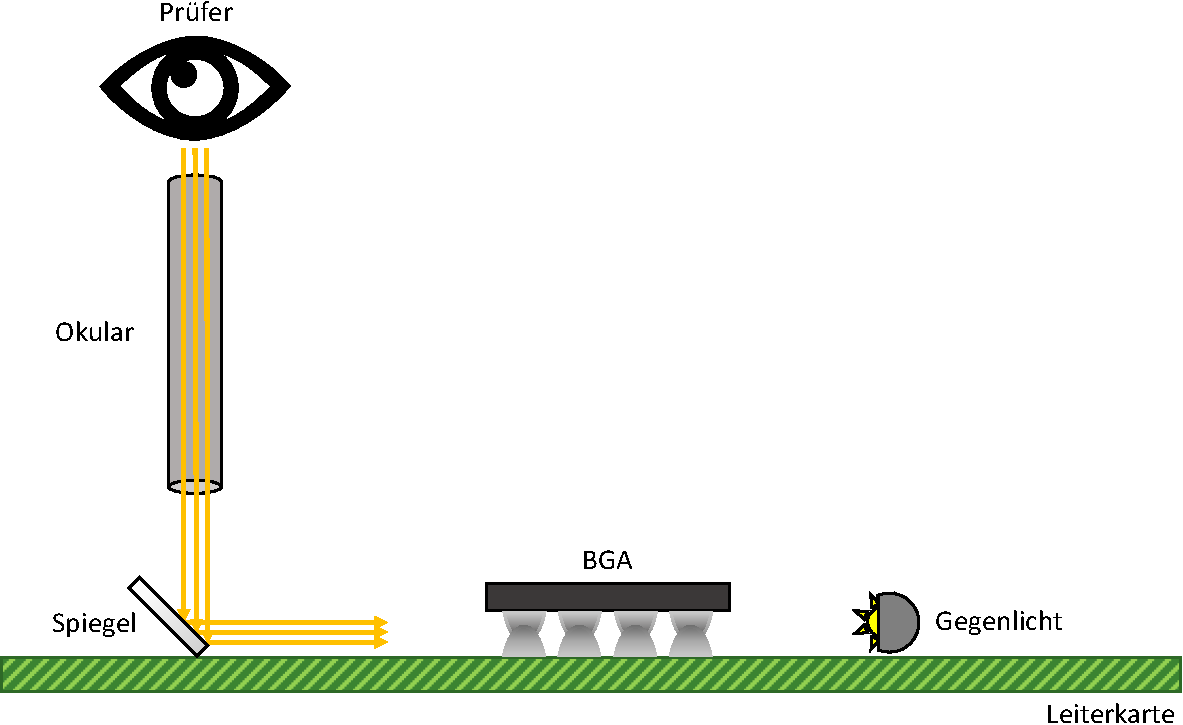
\includegraphics[width = \imgWidth, keepaspectratio = true]{Kapitel/Prüfverfahren in der Elektronikfertigung/Optische Prüfverfahren/Manuelle Optische Inspektion/Grafiken/BGA-InspektionFunktionsweise.pdf}
            \caption[Struktureller Aufbau eines \acs{bga}-Inspektionsgerätes]{Struktureller Aufbau eines \acs{bga}-Inspektionsgerätes. Mithilfe eines Spiegels können die Lötmenisken unterhalb des \acs{bga}-Chips betrachtet werden. In Anlehnung an: \cite{berger_test-_2012}}
            \label{Grafik: BGA-InspektionFunktionsweise}
        \end{figure}

        In der Regel weist dieser Inspektionskopf eine Tiefe von $1,5\,\si{\milli\metre}$ und eine Breite von $5\,\si{\milli\metre}$ bis $6\,\si{\milli\metre}$ auf.
        Die Tiefe ist entscheidend für die Lücke zwischen umliegenden Bauteilen und dem \ac{bga}.
        Die Breite ist ausschlaggebend, um die seitlich verfahrbare maximale Kantenlänge des \ac{bga}-Bausteins betrachten zu können.
        Meistens wird diese Länge durch umliegende Bauelemente limitiert (s. Abbildung \ref{Grafik: BGA-Inspektionsgeraet}). \cite{berger_test-_2012}

        Zur Ausleuchtung der ballförmigen Kontakte wird eine Kombination aus Front- und Gegenlicht verwendet.
        Das Frontlicht ist am Inspektionskopf angebracht und beleuchtet die am Rande und in erster Reihe liegenden Bälle.
        Aufgrund der direkten Beleuchtung ist die Betrachtung der Oberflächenstruktur, der Verbindungen und der Lötmenisken möglich.
        Zusätzlich können die \ac{bga}-Bälle auf Fehler, wie z.B. Mikrorisse, untersucht werden.  \cite{berger_test-_2012}

        Da sich die ballförmigen Kontake bei der Betrachtung gegenseitig optisch verdecken können, wird zusätzlich auch ein Gegenlicht eingesetzt.
        Diese Verdeckung ist in Abbildung \ref{Grafik: BGA-Inspektionsgeraet} in Form der Schatten erkenntlich. \cite{berger_test-_2012}

        \begin{figure}[htbp]
            \centering
            \includegraphics[width = 0.5\imgWidth, keepaspectratio = true]{Kapitel/Prüfverfahren in der Elektronikfertigung/Optische Prüfverfahren/Manuelle Optische Inspektion/Grafiken/BGA-Inspektionsgerät.pdf}
            \caption[Funktionsweise eines \acs{bga}-Inspektionsgerätes]{Funktionsweise eines \acs{bga}-Inspektionsgerätes. Die eingezeichneten Lichtstrahlen zeigen beobachtbare Punkte auf. In Anlehnung an: \cite{berger_test-_2012}}
            \label{Grafik: BGA-Inspektionsgeraet}
        \end{figure}

        Das Gegenlicht hilft bei der kontrastreicheren Darstellung der Form und Kanten innenliegender Lötbälle, da diese sonst aufgrund der Lichtabschottung durch dazwischenliegende Bälle nicht beleuchtet wären.
        Sowohl Front-, als auch das Gegenlicht sind seitlich synchron verfahrbar, sodass die einzelnen Durchgänge der Kontaktreihen nacheinander auf Lötbrücken oder Rückstände hin untersucht werden können. \cite{berger_test-_2012}

        Weiter ist der PC-unterstützte Bildvergleich als Hilfsmittel bei der \ac{moi} zu nennen.
        Zuerst wird das Golden Board und der Prüfling, z.B. mithilfe eines Scanners oder einer Kamera, in das Darstellungsprogramm auf dem Computer eingelesen.
        Dann wird der Prüfling und das Golden Board abwechselnd in einem bestimmten Intervall auf einem Monitor dargestellt.
        Durch den direkten Vergleich werden somit Unterschiede sichtbar dargestellt, die dann von der Prüfperson zu bewerten sind. \cite{berger_test-_2012}

    \minisec{Bewertung}
        Die \ac{moi} hat nach wie vor eine große Bedeutung in der Elektronikfertigung.
        Vorteilhaft ist, dass die \ac{moi} aus der Kategorie der optischen Prüfverfahren die größte Fehlerabdeckung besitzt. 
        Die Kosten, die initial für das Prüfen des Prüflings aufgewendet werden müssen, sind gering, da zum einen die Prüfmittel, wie ein Mikroskop - natürlich in Abhängigkeit der Leistungsfähigkeit - relativ kostengünstig erworben werden können und zum Anderen, da weitere Kosten, z.B. durch das Kaufen von Adaptern, das Anlernen von Personal, oder die Prüfprogrammerstellung wegfallen. \cite{berger_test-_2012}
        Zwar ist statt der Erstellung eines Prüfprogrammes die Erstellung eines Testplanes notwendig, damit keine möglichen Fehlerquellen bei der Kontrolle außer Acht gelassen werden, jedoch ist ein Prüfprogramm weitaus komplexer, da es richtige Eingabeparameter und genaue Instruktionen zur Prüfung braucht.
        Zudem ist der Mensch als lernfähiges Wesen dazu in der Lage, selbst Korrekturen am Prüfprozess anzufertigen, falls z.B. ein Prüfschritt fehlt und durch selbstständiges Handeln und Denken das Wissensrepertoire für weitere Prüflinge zu erweitern, falls ein neuer Fehler gefunden wurde - sozusagen als selbstoptimierender Prüfprozess \cite{berger_test-_2012}.

        Allerdings weist die selbstständige Auffassungsgabe auch einige Nachteile auf, die sich ausschlaggebend auf die Prüfqualität auswirken.
        Aufgrund unterschiedlicher Erfahrungen würde der selbe Prüfling zum Beispiel von zwei Prüfern unterschiedlich streng oder detailliert bewertet werden.
        Da der Prüfprozess aufgrund der manuellen Ausübung langwierig ist und viel Konzentration benötigt, treten bei der Prüfung oft Ermüdungserscheinungen in den Vordergrund, die zu einem großen Fehlerschlupf führen.
        Solche \glqq verschwindenden Fehler\grqq\@ und eine damit gleichzeitig einhergehende Qualitätsminderung entsprechen nicht dem Trend der stetig zunehmenden Zuverlässigkeitsanforderungen (s. Kapitel \ref{subsubsection: Motivation}).
        Die im Vergleich zur einer Maschine langsame Prüfgeschwindigkeit macht eine ausschließliche Nutzung der \ac{moi} nicht effizient, da sie, in der Produktionskette integriert, als das langsamste Glied zum Takttreiber wird.
        Deswegen ist die \ac{moi} nur für stichprobenartige Kontrollen, zur Erhebung einer Statistik dienend, oder zur Korrektur von Fehlern, die durch alternative Testverfahren detektiert worden sind, geeignet. \cite{berger_test-_2012}

        Zusätzlich sollen nun noch einmal die Kosten pro Prüfung beleuchtet werden.
        Da das Prüfverfahren eine ständige und genaue Aufmerksamkeit eines Prüfers voraussetzt, ist dieses sehr personalgebunden, sodass ein Mitarbeiter für einen wohlmöglich langen Zeitraum nicht für andere Aufgaben zur Verfügung steht.
        Gleichzeitig sind durch die aufgewandte Zeit auch die Personalkosten sehr hoch. \cite{berger_test-_2012}
        Diese hohen Personalkosten würden wiederum auf den Prüfling abgewälzt werden, sodass der Produktpreis steigen muss.

    \minisec{\acl{dft}}
        Damit die \ac{moi} bestmöglichst eingesetzt werden kann, müssen in der Entwicklungsphase der Leiterkarte bestimmte Punkte berücksichtigt werden.

        Die notwendige Bedingung ist, dass die auf Fehler zu untersuchenden Stellen auf der Leiterkarte frei sichtbar sein müssen.
        Um dies zu erreichen, sollten sich die Entwickler der Leiterkarte in die Prüfperson hineinversetzen, oder selbst eine Sichtkontrolle durchführen.
        Falls im Laufe des Fertigungsprozesses weitere Bauteile auf die Leiterkarte montiert werden, so bietet sich die prophylaktische Kontrolle der Leiterkarte im vorherigen Produktionsprozess an. \cite{berger_test-_2012}